% !TEX encoding = UTF-8
% !TEX TS-program = pdflatex
% !TEX root = ../tesi.tex

%**************************************************************
\chapter{Progettazione e codifica}
\label{cap:progettazione-codifica}
%**************************************************************

\intro{Breve introduzione al capitolo}\\
Il presente capitolo ha lo scopo di presentare e dimostrare l'architettura per i componenti IW e SP che dovranno funzionare nel contesto dell'estensione del prodotto Monokee.
%**************************************************************
\section{Componente Identity Wallet}
Questa sezione inizia con una generica introduzione all’architettura Xamarin ed si conclude conclude presentando una prima ipotesi di architettura in formato UML 2.0.
\subsection{Tecnologie e strumenti}
\label{sec:tecnologie-strumenti}
Il componente Identity Wallet è sviluppato come applicazione mobile. Questo contesto implica differenti tecnologie che comunicano e interagiscono fra loro. Le funzionalità di persistenza vengono offerte tramite tre diverse tecnologie: file system, blockchain, e server Monokee. La logica di business è implementata usando il framework .NET. L’interfaccia, invece, usa il pattern MVVM (Model View View Model).
L’IW utilizza una classica architettura a strati (N-tier architecture). Trattandosi di un sistema mobile multi piattaforma questa architettura è stata calata nel contesto e quindi si è deciso di basarla sul concetto di Portable Class Libraries (PCL) presentato da Xamarin. 

\subsubsection{Portable Class Libraries PCL}
\gls{pclg}\glsfirstoccur è un approccio alla condivisione del codice tra le diverse edizioni dell’app destinate a diversi sistemi operativi mobili sviluppati da Xamarin. Segue un diagramma esplicativo di come si sviluppa una tipica architettura PCL. Il diagramma in figura \ref{fig:ark-pcl} è tratto da \url{www.xamarin.com}.

\begin{figure}[!h]
    
    \centering
    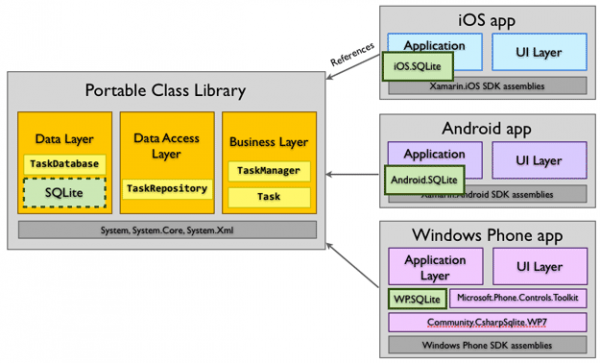
\includegraphics[width=0.9\columnwidth]{ark-pcl.png} 
    \caption{Architettura PCL}
    \label{fig:ark-pcl} 
\end{figure}

Ogni \emph{“Platform-Specific Application Project”} (iOS app, Android app, Windows Phone app) referenzia la \gls{pclg}. Esistono essenzialmente due parti: quelle specifiche per la piattaforma e quelle condivise. Obiettivo del progetto è quello di rendere meno corposa possibile le parti specifiche. Sarà poi possibile impiegare caratteristiche di una determinata piattaforma attraverso l’utilizzo del design pattern \emph{Dependency Injection} (DI).
Applicare i principi della DI significa definire nel codice condiviso interfacce (classi astratte) che vengono implementate (estese) in ogni piattaforma tramite sottoclassi (\emph{Strategy Pattern}). A questo punto sarà possibile integrare le specifiche implementazioni all’interno della PCL. Xamarin per questo scopo offre la classe \emph{DependencyService}.
classi e canali diversi

\subsection{Overview}
Come già detto, l’applicativo è strutturato come una N-tier application consistente dei seguenti layer:
\begin{itemize}
    \item layer presentazione;
    \item logica di business;
    \item layer di accesso ai dati. 
\end{itemize}
    
Quando si sviluppa un’applicazione è importante scegliere se sviluppare un \emph{thin Web-based client} o \emph{un rich client}. Ovviamente, considerando il nostro contesto, ricadiamo nel primo caso, infatti quasi tutta la logica e la persistenza rientrano sul componente ITF. In figura \ref{fig:ark-iw} un'immagine esplicativa dell'architettura ideata.
\begin{figure}[htbp]
    
    \centering
    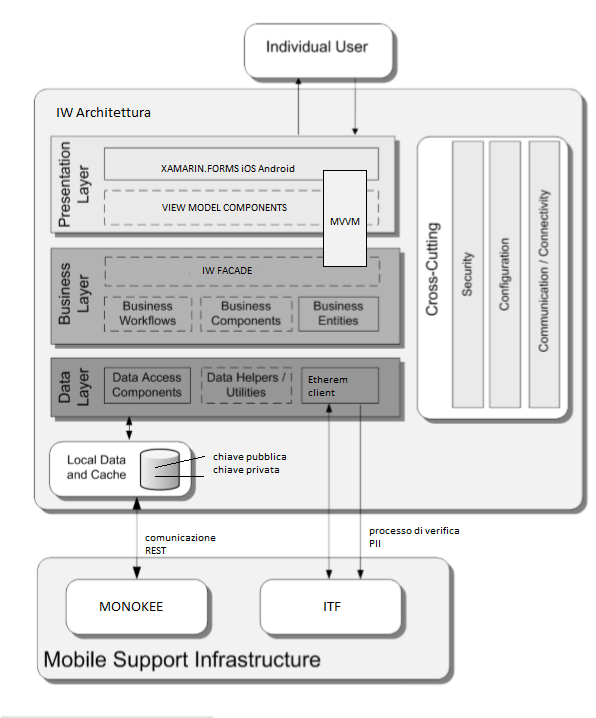
\includegraphics[width=0.9\columnwidth]{ark-iw.png} 
    \caption{Architettura PCWL}
    \label{fig:ark-iw} 
\end{figure}
Come si può notare il principale pattern utilizzato per gestire l’interazione con l’utente è il Model View ViewModel (MVVM). Tutte le elaborazioni vengono effettuate dallo strato di business, mentre per la persistenza ci si affida principalmente alla risorsa Monokee tramite comunicazione REST, oppure all’ITF tramite l’utilizzo di un client Ethereum. Tutto verrà sviluppato utilizzando il framework .NET.

%**************************************************************
\subsection{Progettazione}
\label{sec:progettazione}
In figura \ref{fig:ark-mod-iw} viene presentato il diagramma di massima dell’architettura dell’IW. Il diagramma è stata redatto seguendo lo standard \emph{UML 2.0}. Subito a seguire viene descritta ogni classe.
\begin{figure}[htbp]
    
    \centering
    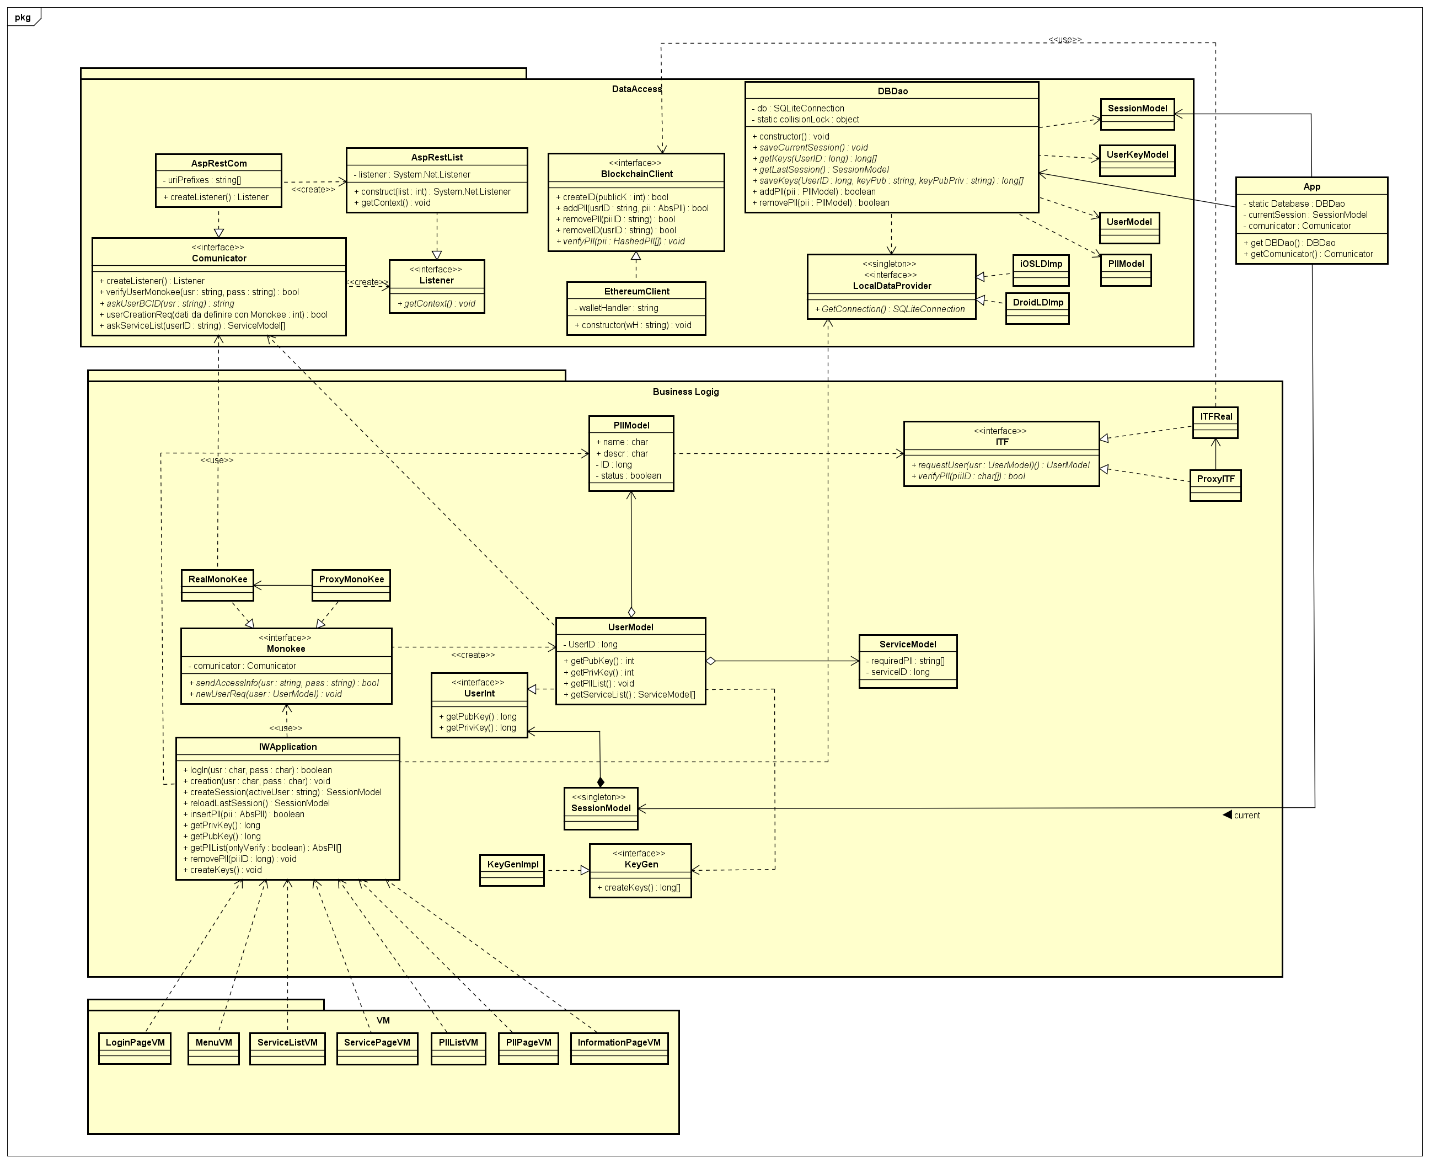
\includegraphics[width=0.9\columnwidth]{iw-complete-uml.png} 
    \caption{Architettura IW}
    \label{fig:ark-mod-iw} 
\end{figure}

\subsubsection{BusinessLogic} %**************************
Nel contesto dell’architettura N-tier adottata, il BusinessLogic layer è un gruppo di classi che si occupa di effettuare e di mantenere tutte le regole definite dai documenti IW - Analisi di massima, IW – Studio di fattibilità.  

\begin{figure}[htbp]
    \centering
    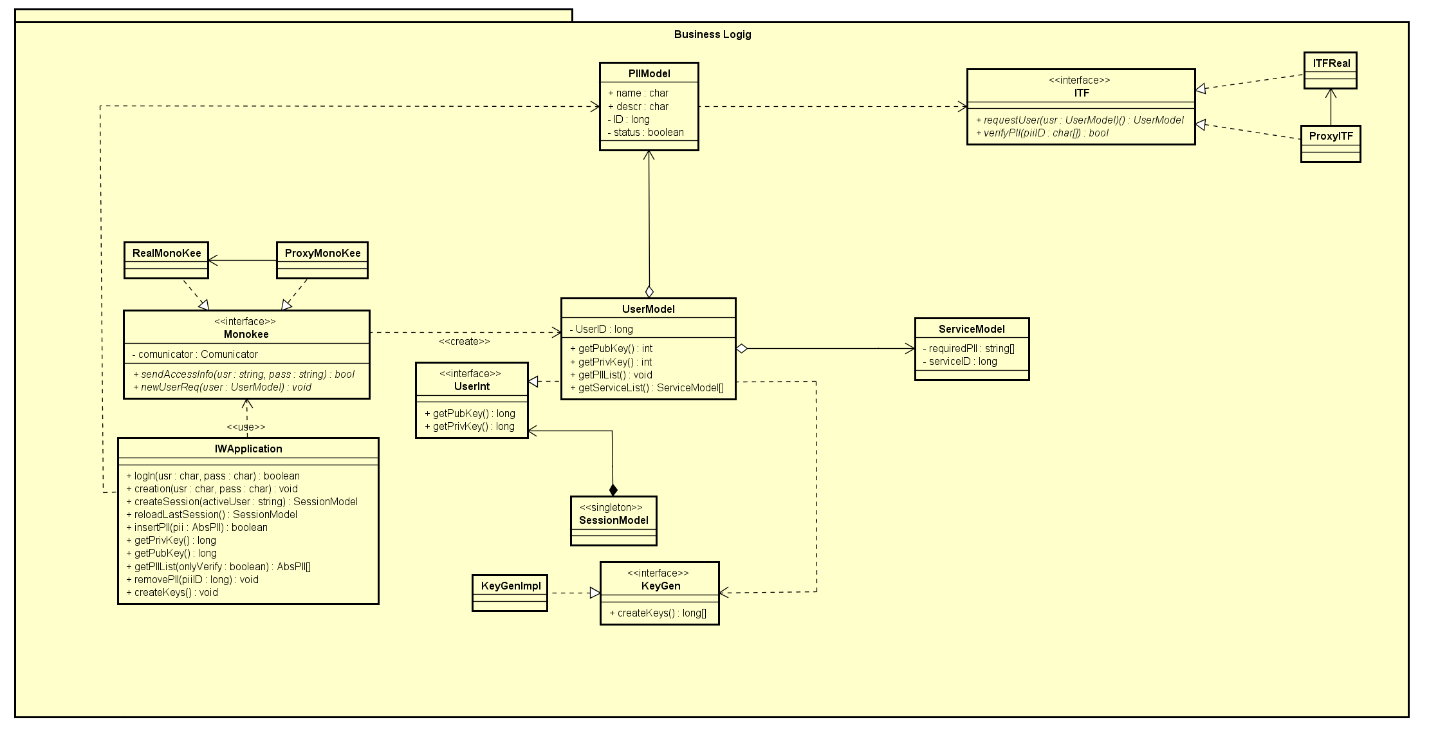
\includegraphics[width=0.9\columnwidth]{bl-lay-iw.png} 
    \caption{Diagramma BusinessLogic Layer IW}
    \label{fig:bl-lay-iw} 
\end{figure}
\begin{namespacedesc}
    \classdesc{IWApplication}{classe che ha il compito di fornire una facade per i vari ViewModel, di conseguenza tutte le azioni possibili tramite l’interfaccia sono implementate da essa.}

    \classdesc{Monokee}{interfaccia che ha il compito di fornire un’astrazione del servizio Monokee. L' interfaccia con RealMonokee e ProxyMonokee rappresenta un’applicazione del pattern Proxy.}

    \classdesc{RealMonokee}{classe che rappresenta il reale oggetto Monokee e che dialoga poi con RESTComp per ottenere i dati. Questa classe con RealMonokee e ProxyMonokee rappresenta un’applicazione del pattern Proxy.}

    \classdesc{ProxyMonokee}{classe che rappresenta un proxy dell’oggetto Monokee, questa classe applica una politica di acquisizione pigra. Questa classe con RealMonokee e ProxyMonokee rappresenta un’applicazione del pattern Proxy.}

    \classdesc{KeyGen}{interfaccia che ha lo scopo di definire una strategia di generazione chiavi. Fa parte di un’applicazione dello Strategy Pattern ed è stata pensata in un’ottica in cui vi possano essere vari modi per generare una chiave a seconda del sistema operativo usato.}

    \classdesc{KeyGenImpl}{classe che rappresenta una possibile implementazione dell’interfaccia KeyGen. Fa parte di un’applicazione dello Strategy pattern.}

    \classdesc{Session}{classe con lo scopo di immagazzinare tutti i dati di una sessione attiva; questa può essere generata dal file system o creata da zero. Deve essere presente in istanza singola e inoltre contiene le informazioni utente.}

    \classdesc{UserInt}{interfaccia che rappresenta un qualsiasi utente dell’applicazione. È implementata solamente da UserMonokee. Questo oggetto viene creato dall’interfaccia Monokee.}

    \classdesc{UserMonokee}{classe che rappresenta un utente proveniente dal server Monokee. Implementa l’interfaccia Monokee. Un utente di questo tipo possiede un aggregato di servizi e una lista PII; potenzialmente può contenere le chiavi.}

    \classdesc{Service}{classe che rappresenta un servizio di cui l’utente ha diritto. Possiede un ID e fornisce una lista di PII che dovranno essere presentati al fine di eseguire l’accesso.}

    \classdesc{KeyProv}{classe che ha il compito di occuparsi della generazione delle chiavi private e pubbliche. Viene usata da UserInt e a sua volta usa LocalDataProvider.}

    \classdesc{LocalDataProvider}{interfaccia che ha il compito di fornire in singolo punto dove ottenere informazione dal file system locale. Successivamente deve essere implementata in base al sistema operativo su cui girerà. }

    \classdesc{iOSLDImp}{rappresenta l’implementazione per iOS di LocalDataProvider.}

    \classdesc{DroidLDImp}{rappresenta l’implementazione Android di LocalDataProvider.}

    \classdesc{AbsPII}{interfaccia che rappresenta una generica PII. Ha una sola possibile implementazione, ma PUò rendere più semplice l’implementazione di future PII.}

    \classdesc{PIIImpl}{classe che rappresenta l’attuale ed unica PII. Consiste di un nome, un identificativo e una descrizione. Una PII può essere verificata o meno tramite l’uso di PIIChecker. }

    \classdesc{ITF}{interfaccia che ha il compito di fornire un’astrazione del componente Identity Trust Fabric. Con ITFReal e ProxyITF rappresenta un’applicazione del pattern Proxy.}
    \classdesc{RealITF}{classe che rappresenta il reale oggetto ITF. Essa dialoga poi con il BlockchainClient per ottenere i dati. Con RealITF e ProxyITF rappresenta un’applicazione del pattern Proxy.}
    \classdesc{ProxyITF}{classe che rappresenta un proxy dell’oggetto Monokee, questa. Applica una politica di acquisizione pigra. Con RealITF e ProxyITF rappresenta un’applicazione del pattern Proxy.}
    \classdesc{PIIChecher}{classe che ha il compito di verificare tramite ITF la veridicità di una PII.}
\end{namespacedesc}

\subsubsection{DataAccess Layer} %**************************
Nel contesto dell’architettura N-tier adottata il \emph{DataAccess} layer è un gruppo di classi che si occupano di interfacciarsi con gli strumenti di persistenza utilizzati dall’applicazione. Questi sono: Monokee (tramite RESTful), ITF e una base di dati locale al dispositivo. 
\begin{figure}[htbp]
    \centering
    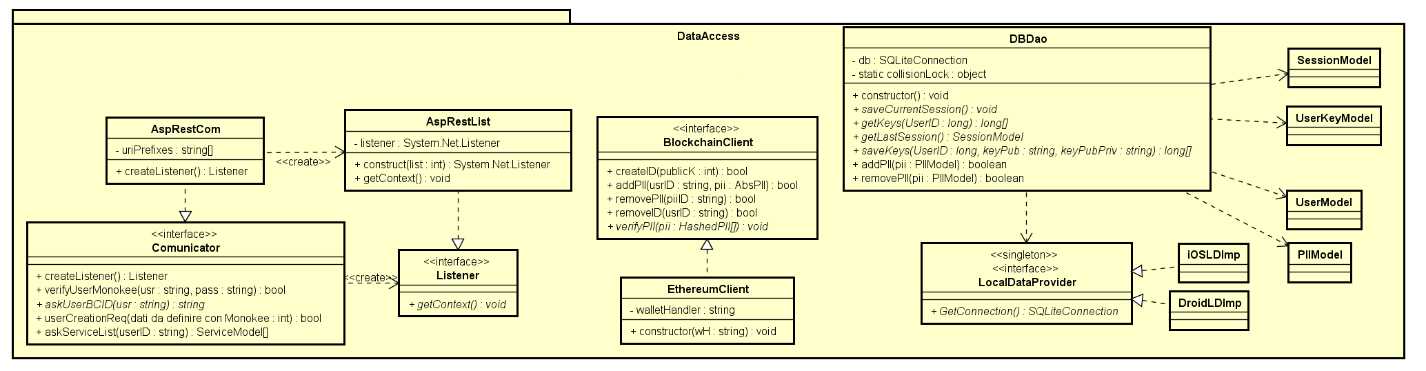
\includegraphics[width=0.9\columnwidth]{dla-iw.png} 
    \caption{Diagramma DataAccess Layer IW}
    \label{fig:dla-iw} 
\end{figure}

\begin{namespacedesc}
    \classdesc{RestComp}{interfaccia che ha il compito di rappresentare una generica strategia di comunicazione REST. Essa viene utilizzata da RealMonokee per ottenere i dati relativi all’utente.}
    \classdesc{RestImpl}{possibile implementazione della strategia di comunicazione REST. Implementa l’interfaccia RestComp.}
    \classdesc{BlockchainClient}{interfaccia che ha il compito di rappresentare una generica strategia di comunicazione con la rete blockchain. Questa astrazione permette di slegare dall’architettura dipendenze con le varie implementazioni di blockchain e anche di client.}
    \classdesc{EthereumClient}{possibile implementazione di BlockchainClient che utilizza la rete Ethereum. Questa classe poi userà la libreria Nethereum.}
\end{namespacedesc}



\subsubsection{PresentationLayer} %**************************
Questo layer contiene i vari controllori che gestiscono le viste. Si è previsto di creare un controller per ogni pagina dell’applicazione. L’applicazione utilizza il pattern MVVM, quindi, i controlli sono delle ViewModel (VM) che contengono i dati e le operazioni. Tra i dati e la vista sono presenti dei binding da realizzare utilizzando gli strumenti forniti da Xamarin. Le VM operano le loro azioni tramite l’utilizzo della classe IWFacade. 


Tutte queste classi devono estendere da INotifyPropertyChanged.
In figura \ref{fig:vm-layer-iw} il diagramma esplicativo del \emph{layer}.

\begin{figure}[htbp]
    \centering
    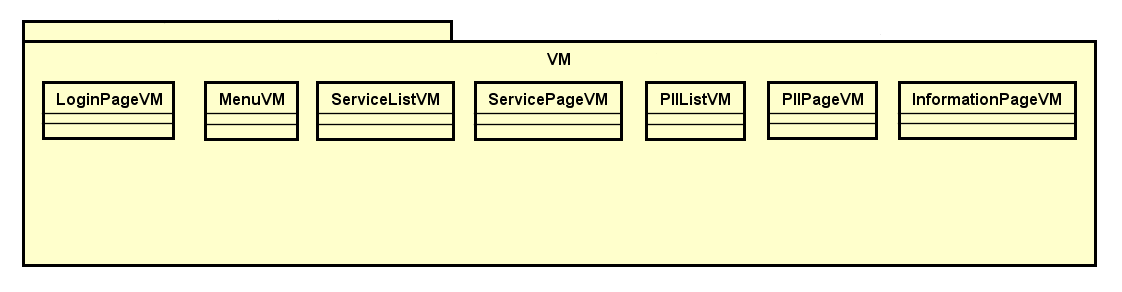
\includegraphics[width=0.9\columnwidth]{VMlayer-iw.png} 
    \caption{Diagramma UML VM Layer}
    \label{fig:vm-layer-iw} 
\end{figure}

\begin{namespacedesc}
    \classdesc{LoginPageVM}{classe che ha lo scopo di gestire la pagina di log in e quindi avere lo stato e le operazioni necessarie.}
    \classdesc{MenuVM}{classe che ha lo scopo di gestire il menù dell’applicazione e quindi avere lo stato e le operazioni necessarie.}
    \classdesc{ServiceListVM}{classe che ha lo scopo di gestire la pagina che presenta la lista dei service a cui può accedere l’utente e quindi avere lo stato e le operazioni necessarie.}
    \classdesc{ServicePage}{classe che ha lo scopo di gestire la pagina con le informazioni relative ad un singolo servizio e quindi avere lo stato e le operazioni necessarie.}
    \classdesc{PIIListVM}{classe che ha lo scopo di gestire la pagina che presenta la lista delle PII che possiede l’utente e quindi avere lo stato e le operazioni necessarie.}
    \classdesc{PIIPageVM}{classe con lo scopo di gestire la pagina che visualizza le informazioni relative ad una specifica PII e quindi avere lo stato e le operazioni necessarie.}
    \classdesc{InformationPageVM}{classe che ha lo scopo di gestire la pagina che fornisce le informazioni sull’applicazione, sul servizio Monokee e le istruzioni per l’uso.}
\end{namespacedesc}
%**************************************************************
\subsection{Design Pattern utilizzati}
Al fine di garantire elevate doti di qualità e manutenibilità dell’architettura sono stati usati una serie di design pattern. Di seguito segue una breve descrizione di questi.

\paragraph{Communicator}: incapsula i dettagli interni della comunicazione in un componente separato che poi può essere implementato usando tecnologie diverse; risultato utile per rendere gli altri componenti quanto più indipendenti da come comunicano con l’esterno.

\paragraph{Data Transfer Object (DTO)}: oggetto che ha il compito di racchiudere le informazioni utili a diverse componenti. Va a ridurre i metodi necessari per la comunicazione e, in generale, la semplifica.

\paragraph{Entity Translator}: oggetto che trasforma un dato in forma utile per essere usato nella logica di business. Esso è stato usato per interfacciarsi con il client Ethereum e il server Monokee.

\paragraph{Lazy Acquisition Proxy}: Ritarda l’acquisizione delle risorse il più a lungo possibile. Esso è stato ampiamente utilizzato, specialmente per rendere più leggera possibile la creazione dei dati dell’utente e della verifica dei dati nell’ITF.

\paragraph{Strategy Pattern}: oggetto che permette di separare l’esecuzione di un metodo dalla classe che lo contiene. Usando un’interfaccia per astrarre il metodo è poi possibile creare molteplici implementazioni. Ciò è risultato molto utile nel contesto di un’applicazione multi piattaforma in cui alcune procedure dovevano essere implementate in nativo. Oltretutto ha reso possibile separare il metodo dall’implementazione.

\paragraph{Dependency Injection}: pattern che permette di delegare il controllo della creazione oggetti ad un oggetto esterno. Esso permette di semplificare la gestione delle dipendenze e, nel contesto dello strategy pattern, permette di inserire l’implementazione corretta.

\paragraph{Model-View-Controller}: separa il codice per l’interfaccia grafica in tre componenti separati: Modello (il dato), Vista (l’interfaccia), and Controllore (il responsabile della logica), con particolare attenzione alla vista. Nel progetto viene usata una sua particolare declinazione chiamata MVVM. 

%**************************************************************


%COMPONENTE SP ********************************************************************
\newpage
\section{Componente Service Provider}
La sezione inizia con una generica introduzione alle architetture Event Driven. Si è deciso di utilizzare un approccio Broken topology; la scelta è motivata dalla maggior indipendenza tra i vari componenti rispetto ad un approccio Mediator topology. Infine si conclude con la presentazione una prima ipotesi di architettura in formato UML 2.0.



\subsection{Tecnologie e strumenti}
\label{sec:tecnologie-strumenti}
Il componente Service Provider è sviluppato come applicazione server, questo implica possibili accessi multipli al servizio da parte di vari Real Service Provider (RSP) che inoltrano le loro richieste di accesso. L’applicativo fa uso di diverse fonti per espletare le proprie funzioni. Più dettagliatamente queste sono: Monokee, RSP e ITF. Da questo primo studio architetturale non sembrerebbe necessario l’uso di una base di dati locale.  Considerato quanto appena detto si è ritenuta particolarmente adatta un’architettura Event Driven basata sull’utilizzo di code. Per la comunicazione con il RSP e con Monokee si è deciso di utilizzare un approccio basato sulle API RESTful. Invece per la comunicazione verso l’ITF si è deciso di utilizzare un client Ethereum.

\subsubsection{Architettura Event Driven}
Questo tipologia di architettura rappresenta uno dei principali esempi di pattern architettura asincrono. Produce applicati altamente scalabili e facilmente adattabili ad ogni carico di utilizza. Se applicata bene fornisce la possibilità di avere eventi con un singolo scopo (\gls{srpg}\glsfirstoccur) e con un basso livello di accoppiamento. Questo è reso possibile dalla gestione asincrona di questi eventi.
Ci sono due possibili approcci a questa architettura:
\begin{itemize}
    \item Mediator topology;
    \item Broker topology.
\end{itemize}
\subsubsection{Mediator topology}
Un evento generalmente possiede una serie di passi ordinati per essere eseguito. In questa approccio ci sono quattro componenti che interagiscono fra loro:
\begin{itemize}
    \item una o più code di eventi;
    \item un mediatore di eventi;
    \item uno o più esecutori di eventi;
    \item dei canali di eventi.
\end{itemize}
    
Gli eventi possono essere di due tipi:
\begin{itemize}
    \item eventi iniziali;
    \item eventi di processamento.
\end{itemize}
    
In figura \ref{fig:eventdriver-med-top} si riporta una generica architettura \emph{Event Driven Mediator Topology}.   
\begin{figure}[htbp]
    \centering
    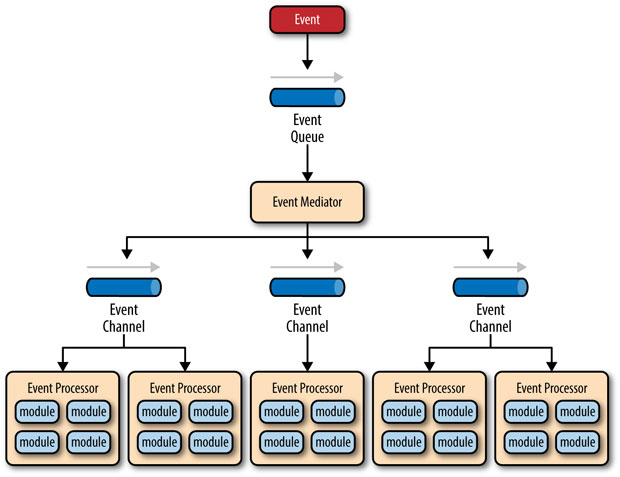
\includegraphics[width=0.9\columnwidth]{med-topology.jpg} 
    \caption{Schema Mediator Topology}
    \label{fig:eventdriver-med-top} 
\end{figure}

\paragraph{Mediatore di eventi}
Il mediatore (l’Event Mediator) ha il compito di orchestrare i passi necessari per rispondere ad un evento iniziale; per ogni passo invia uno specifico evento di processamento ad un canale (Event Channel). Il mediatore non applica nessun tipo di logica, conosce solo i passi necessari per gestire l’evento iniziale e quindi li genera.
\paragraph{Canale di eventi}
Si tratta generalmente di un canale di comunicazione asincrono. Questo può essere di due tipi:
\begin{itemize}
    \item coda di messaggi;
    \item topic di messaggi.
\end{itemize}
\paragraph{Esecutore di eventi}
Contiene la vera logica di business per processo ogni evento. Sono auto contenuti, indipendenti ed scarsamente accoppiati.



\subsubsection{Broker topology}
In questo approccio non è presente un mediatore centrale. Il flusso dei messaggi viene distribuito dai vari esecutori, creando una catena di eventi che generano a loro volta altri eventi. Risulta molto utile nel caso in cui il flusso sia molto semplice. 

In questo approccio ci sono due principali componenti:
\begin{itemize}
    \item un broker che contiene tutti i canali;
    \item vari esecutori di eventi.
\end{itemize}
    
In figura \ref{fig:eventdriven-bro-top} si riporta una generica architettura Event Driven Broker Topology.

\begin{figure}[htbp]
    \centering
    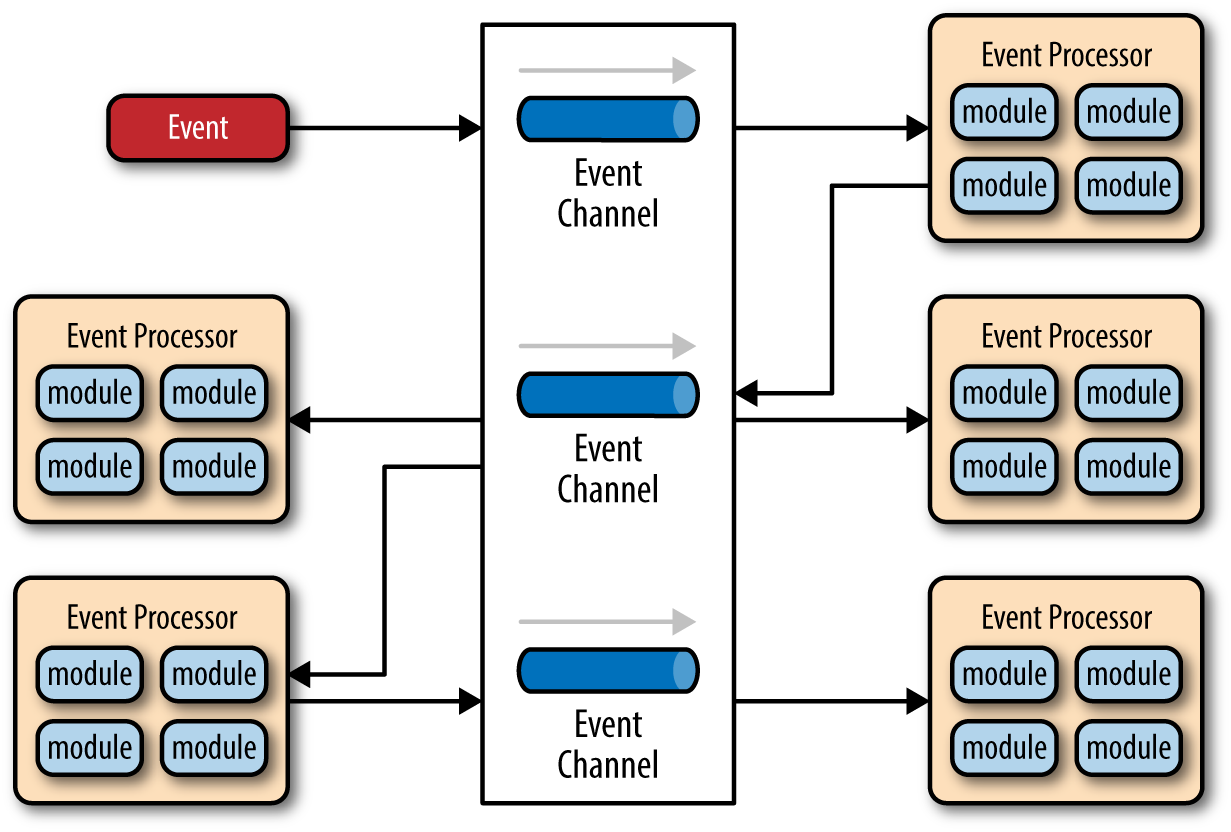
\includegraphics[width=0.9\columnwidth]{brok-top.png} 
    \caption{Schema Broker Topology}
    \label{fig:eventdriven-bro-top} 
\end{figure}

\subsubsection{Considerazioni}
Di seguito si evidenziano alcune vantaggi e svantaggi in maniera analitica \footnote{site:event-driven}:
\paragraph{Agilità generale}
I cambiamenti sono generalmente isolati e possono essere fatti velocemente con piccoli impatti.
\paragraph{Facilità di deploy}
È dovuta all’alto disaccoppiamento degli esecutori. Questa nota vale particolarmente per la tipologia Broker in quanto non presenta il mediatore.
\paragraph{Testabilità}
Richiede strumenti specializzati per generare eventi, questo potrebbe rendere i test di sistema difficoltosi. I test di unità invece sono facilmente implementabili. 
\paragraph{Scalabilità}
La natura indipendente dei componenti rende facile scalare questi in base alle necessità permettendo così un tuning delle risorse molto fine.
\paragraph{Facilità di sviluppo }
È il principale svantaggio di queste architettura.


Uno dei principali svantaggi di questo tipo di architettura è la complessità di implementazione, dovuta al fatto che operazioni sono completamente asincrone e concorrenti. Si è comunque ritenuta questa architettura nella sua variante Broker Topology adatta allo scopo soprattutto per questioni di performance, scalabilità e facilità di deploy.

\subsection{Overview}
Come già detto l’applicazione sarà strutturata con una architettura Event Driven di tipo Broker topology, questo implica che la logica di funzionamento sia incapsulata nei vari passaggi tra le varie code.
Gli esecutori sono i seguenti cinque:
\begin{itemize}
    \item \textbf{Starter}: con il compito di ascoltare gli eventi iniziali dei vari RSP e di ricevere i vari dati ottenuti tramite codici QR;
    \item RetriveInfo: con il compito di ottenere le informazioni necessarie da Monokee;
    \item \textbf{PageResponce}: con il compito di generare e visualizzare le pagine nel broswer dell’utente, sia di fallimento che di comunicazione;
    \item \textbf{PiiDataHandler}: con il compito di verificare i dati nell’ITF e verificare che questi siano sufficienti per effettuare l’accesso;
    \item \textbf{RSPSendingWork}: con il compito di inviare al RSP le informazioni di accesso.
\end{itemize}
    
Gli eventi sono i seguenti:
\begin{itemize}
    \item \textbf{AccessRequest}: generato dallo starter e eseguito dal RetriveInfo;
    \item \textbf{PageResponce}: generato dal RetriveInfo in caso di errore o per mostrare il lettore QR, dal PiiDataHandler in caso di login o in caso di insuccesso della verifica;
    \item \textbf{VerificationWork}: generato dallo Starter per verificare i dati forniti tramite il QR e quelli forniti da RequireInfo siano conformi e verificati; 
    \item \textbf{RSPSendingWork}: generato da PiiDataHandler in caso di verifica positiva.
\end{itemize}
    
 Il diagramma in figura \ref{fig:eventdriven-flusso-code} rappresenta come i vari eventi di lavoro si distribuiscono tra i vari esecutori.

 \begin{figure}[!h]
    \centering
    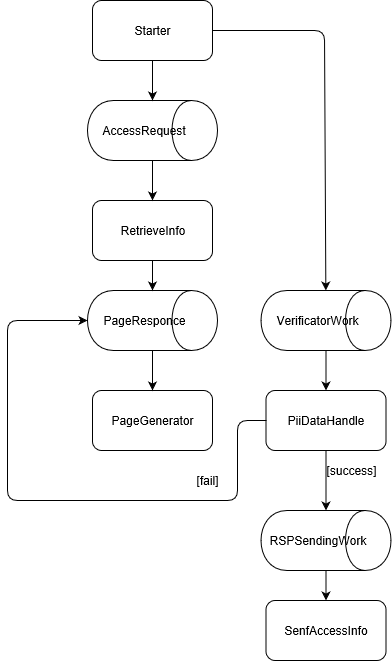
\includegraphics[width=0.7\columnwidth]{flow-eventi-sp.png} 
    \caption{Flusso eventi SP}
    \label{fig:eventdriven-flusso-code} 
\end{figure}
Lo \emph{Starter} quando riceve una richiesta d’accesso da parte del RSP procede a generare il lavoro di \emph{AccessRequest}, una volta ricavati tutti i dati necessari per l’accesso da Monokee, viene affidato al \emph{PageResponce} l’incarico di visualizzare la pagina che richiede l’inserimento del QR. I dati verranno poi inseriti dall’utente e attraverso lo \emph{Starter} verrà creato un lavoro di verifica dei dati inseriti e se questi sono sufficienti ad accedere al servizio, tramite un’ulteriore accesso a Monokee. In caso di esito positivo viene creato un lavoro di invio dati verso il RSP altrimenti verrà visualizzata una pagina di errore.
%**************************************************************

%**************************************************************
\newpage
\subsection{Progettazione}
\label{sec:progettazione}
In figura \ref{fig:sp-uml-diag} si presenta un diagramma delle classi che attua la gestione delle code sopra espletata. Il diagramma è stato redatto in formato \emph{UML 2.0}, con leggere modifiche relativo alla rappresentazione delle varie istanze del template \emph{CommandQueue}. Questo è stato fatto al fine di rendere più leggibile e comprensibile il diagramma. Come si può notare sono presenti componenti non presenti nella precedente trattazione. Questi servono per effettuare le comunicazioni con l’ambiente esterno. Si è deciso per questioni di semplicità di non creare code separate.

\begin{figure}[!htbp]
    \centering
    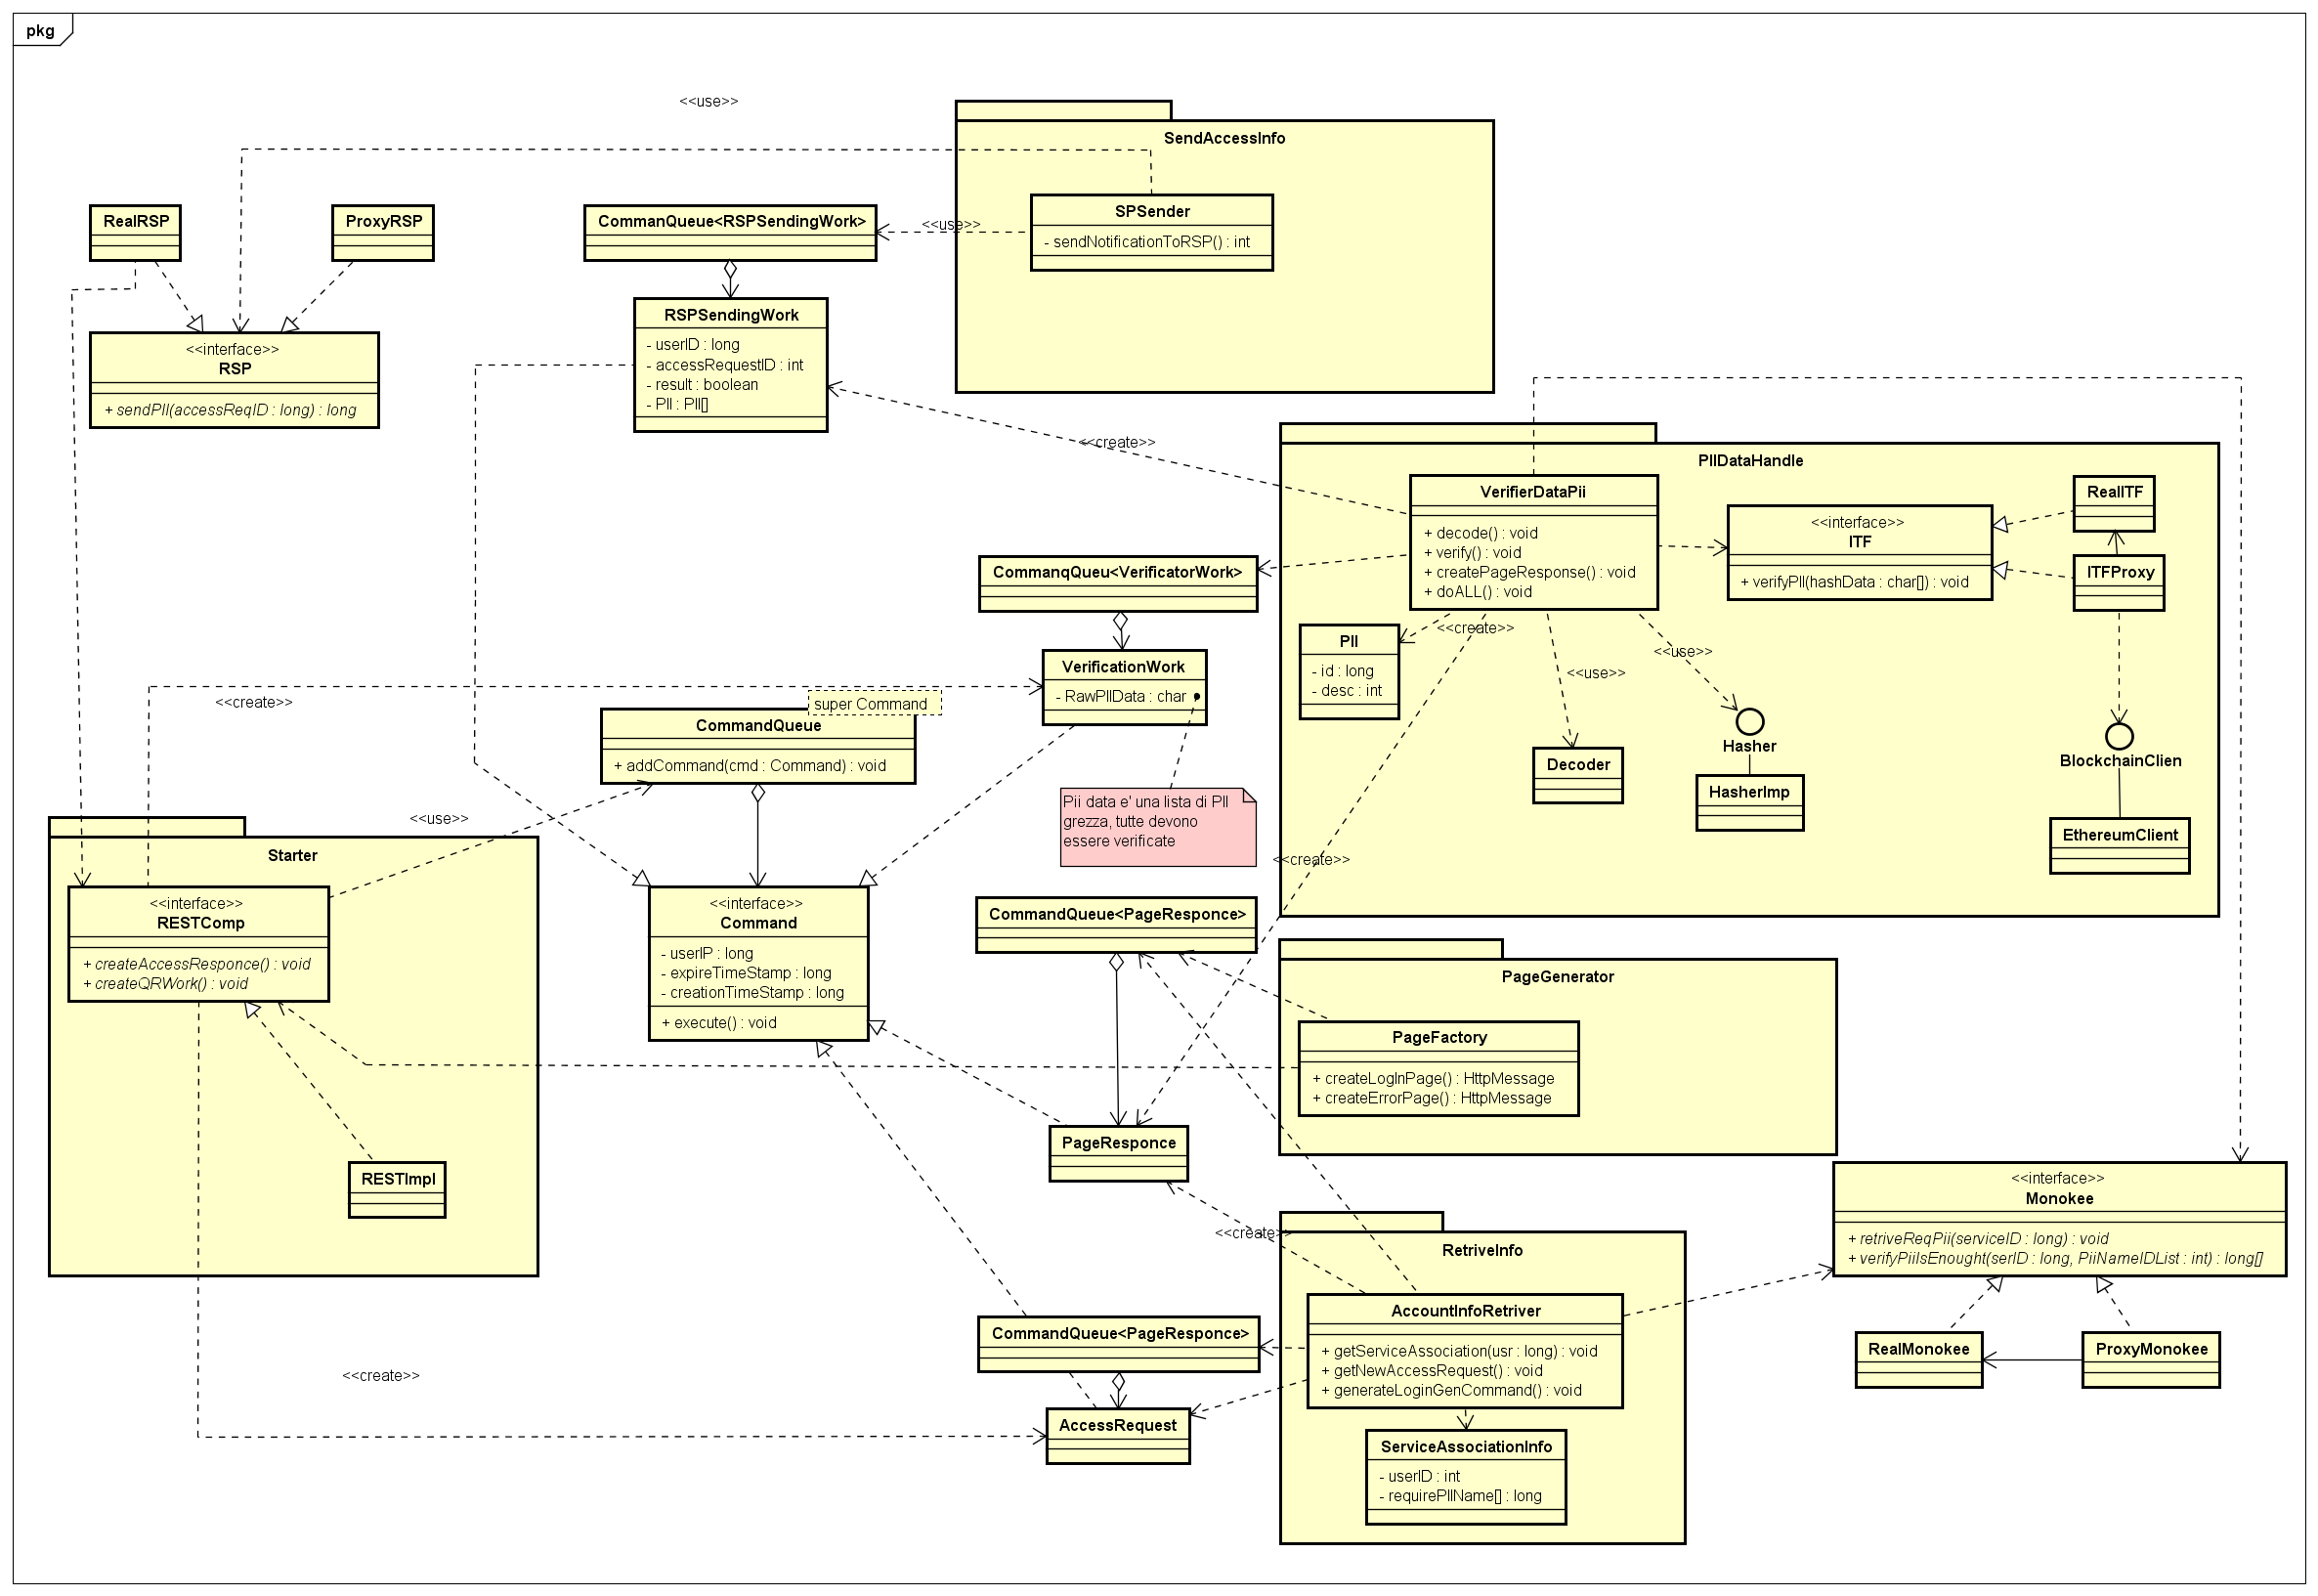
\includegraphics[width=0.9\columnwidth]{SPdiagram.png} 
    \caption{Diagramma delle classi del modulo SP}
    \label{fig:sp-uml-diag} 
\end{figure}

\subsubsection{Starter}
Lo \emph{Starter} rappresenta l’esecutore iniziale. Questo rimane in ascolto di eventuali richieste di accesso inoltrate dagli \emph{RSP} e da inizio all’esecuzione di questa. Riceve inoltre i dati provenienti dai codici QR. In figura \ref{fig:starter-uml-diag} viene riportato il diagramma UML dell'esecutore. Le classi più significative sono di seguito descritte.
\begin{figure}[htbp]
    \centering
    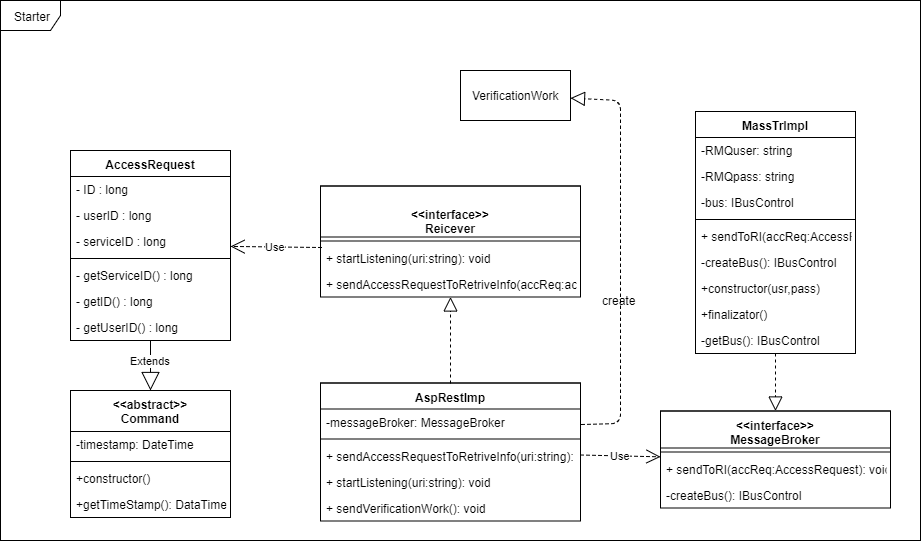
\includegraphics[width=0.9\columnwidth]{starter-uml.png} 
    \caption{Rappresentazione UML di \emph{Starter}}
    \label{fig:starter-uml-diag} 
\end{figure}
\begin{namespacedesc}
    \classdesc{Reicever}{è un'interfaccia con il compito di ricevere le comunicazioni provenienti dal sito di login e, quindi, inoltrare i messaggi alla coda successiva (\emph{RetrieveInfo}). Rappresenta il \emph{driver} del componente \emph{Starter}.}
    \classdesc{AspRestImpl}{è una possibile implementazione della strategia di comunicazione tramite \emph{REST}. Implementa l’interfaccia \emph{Reicever}.}
    \classdesc{MessageBroker}{è un'interfaccia con il compito di definire i metodi necessari alla gestione dalla rete di comunicazione \emph{RabbitMQ}.}
    \classdesc{MassTransitImpl}{questa classe implementa il MessageBroker utilizzano la libreria MassTransit.}
\end{namespacedesc}

\subsubsection{RetriveInfo}
È l’esecutore con il compito di ottenere le informazioni necessarie da \emph{Monokee}. In caso di associazione presente manda il lavoro di creazione pagina di login, in caso di associazione non presente manda il lavoro di creazione pagina di errore.
In figura \ref{fig:retrive-info-uml-diag} viene riportato il diagramma UML dell'esecutore. Le classi più significative sono di seguito descritte.
\begin{figure}[htbp]
    \centering
    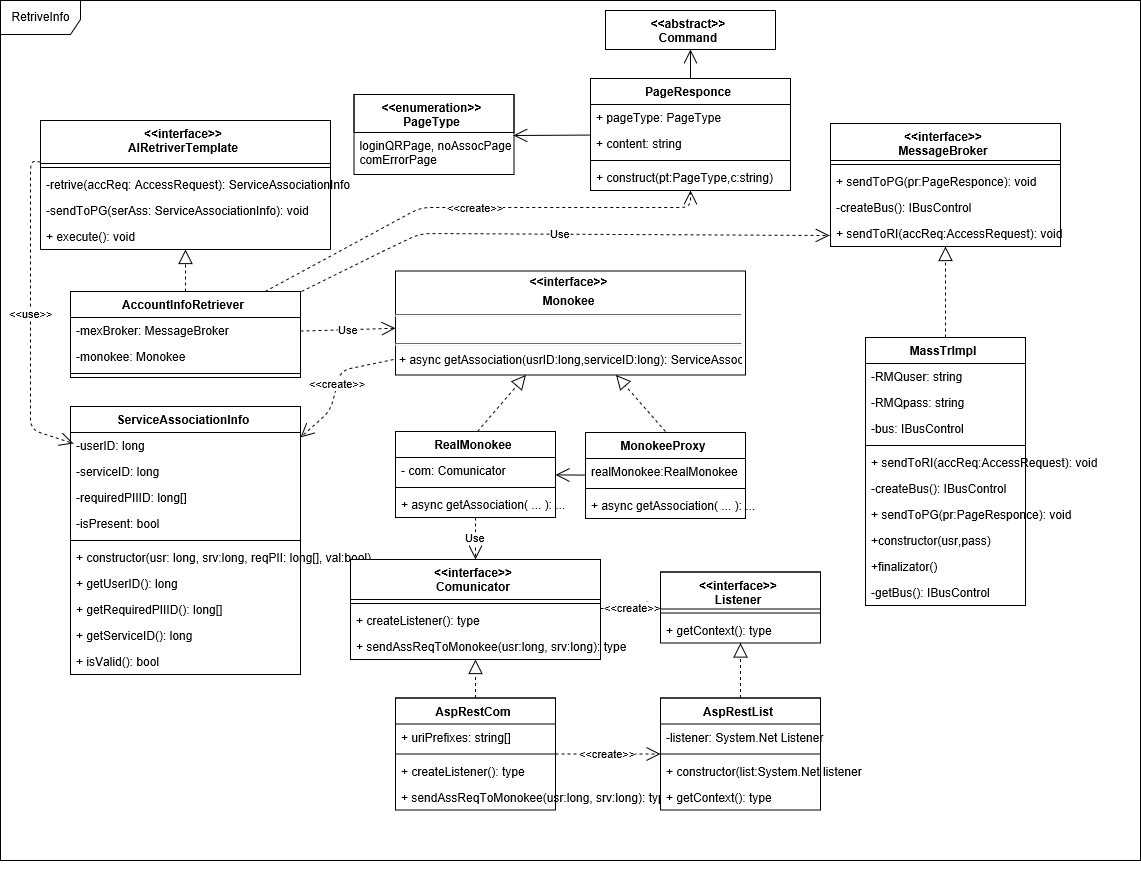
\includegraphics[width=0.9\columnwidth]{retrive-info-uml.png} 
    \caption{Rappresentazione UML di \emph{RetriveInfo}}
    \label{fig:retrive-info-uml-diag} 
\end{figure}
\begin{namespacedesc}
    \classdesc{AIRetriverTemplate}{questa interfaccia ha lo scopo di ricevere gestire e inoltrare i messaggi alla coda successiva (\emph{RetrieveInfo}). Rappresenta un template (\emph{Templete pattern}) del \emph{driver} dell’esecutore \emph{RetriveInfo}.}
    \classdesc{AccountInfoRetriever}{implementazione di \emph{AIRetriverTemplate}.}
    \classdesc{ServiceAssociationInfo}{questa classe rappresenta le informazioni ottenute da \emph{Monokee}, riporta i dati della \emph{AccessRequest} che l’ha generata e ci aggiunge l’informazione relativa alla lista delle \emph{PII} richieste e la presenta o meno della associazione in \emph{Monokee}. È un oggetto immutabile.}
    \classdesc{PageType}{Questo \emph{enumeration} definisce le varie possibili pagine creabili dall’esecutore \emph{PageGenerator}.
    I possibili tipi sono:
    \begin{itemize}
        \item loginQRPage: è una pagina mostra cattura il codice QR con le informazioni necessarie;
        \item noAssocPage: è una pagina che comunica che l’utente che ha effettuato una richiesta per un servizio a cui non è abilitato (non possiede l’associazione in Monokee);
        \item comErrorPage: è una pagina che comunica un generico errore di comunicazione.
    \end{itemize}}
    \classdesc{Monokee}{si tratta di un’interfaccia con il compito di fornire un’astrazione del servizio Monokee. Questa interfaccia con RealMonokee e ProxyMonokee rappresenta un’applicazione del pattern Proxy.}

    \classdesc{RealMonokee}{è una classe che rappresenta il reale oggetto Monokee, questa classe poi dialoga con RESTComp per ottenere i dati. Questa classe con RealMonokee e ProxyMonokee rappresenta un’applicazione del pattern Proxy.}

    \classdesc{ProxyMonokee}{è una classe che rappresenta un proxy dell’oggetto Monokee, questa classe applica una politica di acquisizione pigra. Questa classe con RealMonokee e ProxyMonokee rappresenta un’applicazione del pattern Proxy}

    \classdesc{Comunicator}{questa classe fornisce un’interfaccia per gestire tutte le informazioni attraverso fonti esterne. Deve essere usata per comunicare con \emph{Monokee} e il \emph{Real Service Provider}.}
    \classdesc{AspRestCom}{questa classe implementa \emph{Comunicator} tramite l'utilizzo della libreria \emph{Asp.NET}.}

    \classdesc{Listener}{È un'interfaccia con il compito di rimanere in ascolto su determinati uri. È un oggetto non mutabile.}
    \classdesc{AspRestList}{È un oggetto con il compito di rimanere in ascolto su determinati uri. È un oggetto non mutabile. Questa classe è un \emph{wrapper} del \emph{listener} di \emph{System.Net}. Implementa \emph{Listener}.}
\end{namespacedesc}


\subsubsection{PageGenerator}
È l’esecutore con il compito di ascoltare le richieste di creazione pagina provenienti dagli altri esecutori e quindi di generarle come richiesto e di inviarle al \emph{browser}del richiedente. In figura \ref{fig:pagegenerator-uml-diag} viene riportato il diagramma UML dell'esecutore. Le classi più significative sono di seguito descritte.
\begin{figure}[htbp]
    \centering
    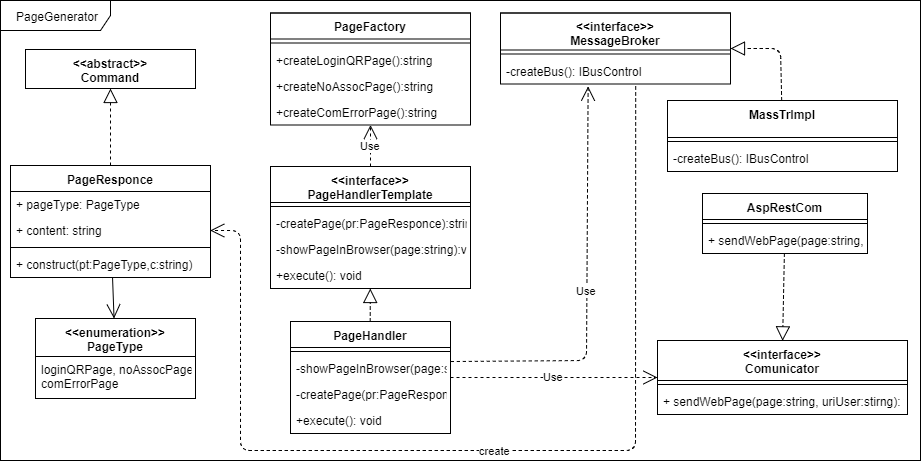
\includegraphics[width=0.9\columnwidth]{pagegenerator-uml.png} 
    \caption{Rappresentazione UML di \emph{PageGenerator}}
    \label{fig:pagegenerator-uml-diag} 
\end{figure}
\begin{namespacedesc}
    \classdesc{PageHandlerTemplate}{questa interfaccia consiste in un \emph{template} per la creazione di un \emph{driver} per la gestione e l’esecuzione dei \emph{Command} di \emph{PageGenerator}.}
    \classdesc{PageHandler}{Questa classe implementa la struttura fornita da \emph{PageHandlerTemplate}.}
\end{namespacedesc}

\subsubsection{PIIDataHandler}
Questo esecutore ha il compito di ricevere nella propria coda dallo \emph{Starter} una serie di lavori di verifica e quindi di verificare questi sia verso \emph{Monokee} sia verso l’\emph{ITF}. In questo esecutore sono presenti le interfacce \emph{Command}, \emph{Monokee} e \emph{MessageBroker} che non verranno presentate. In figura \ref{fig:piidatahandler-diag} viene riportato il diagramma UML dell'esecutore. Le classi più significative sono di seguito descritte. 
\begin{figure}[htbp]
    \centering
    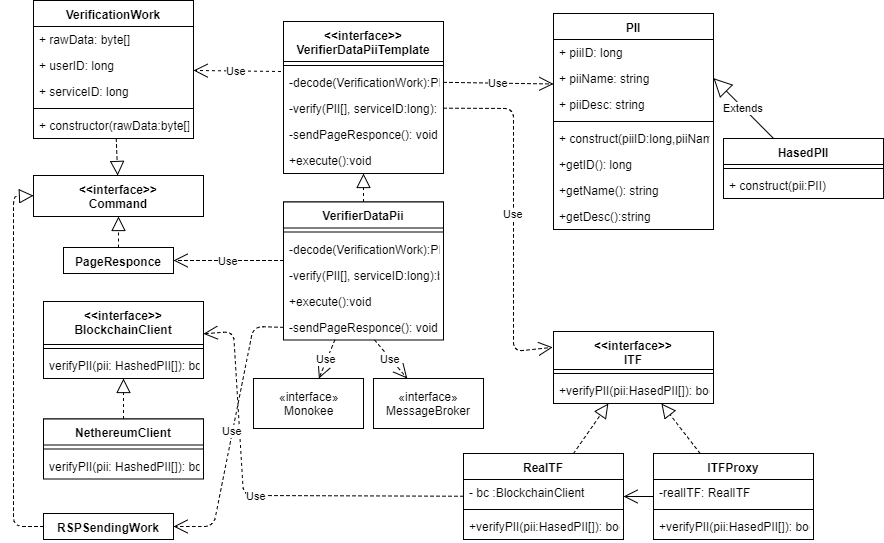
\includegraphics[width=0.9\columnwidth]{piidatahandler-uml.png} 
    \caption{Rappresentazione UML di \emph{PIIDataHandler}}
    \label{fig:piidatahandler-uml-diag} 
\end{figure}

\begin{namespacedesc}
    \classdesc{VerificationDataPiiTemplate}{questa interfaccia rappresenta il \emph{template} da seguire per eseguire l’algoritmo di gestione di un \emph{VerificationPiiWork}. Dalla ricezione fino al suo esaurimento.}
    \classdesc{VerificationDataPii}{Questa classe rappresenta un’applicazione del \emph{template} da seguire per eseguire l’algoritmo di gestione di un \emph{VerificationPiiWork}. Dalla ricezione fino al suo esaurimento.}
    \classdesc{PII}{è una classe che rappresenta una PII. Contiene l’id, la descrizione di una PII.}
    \classdesc{HashedPII}{questa classe rappresenta una \emph{PII} con le informazioni \emph{piiName} e \emph{piiDesc} sotto forma di \emph{Hash}, questa classe dev’essere usata per comunicare con l’\emph{ITF}. L’oggetto è immutabile.}
    \classdesc{ITF}{si tratta di un’interfaccia con il compito di fornire un’astrazione del componente ITF. Questa interfaccia con RealITF e ProxyITF rappresenta un’applicazione del pattern Proxy.}

    \classdesc{RealITF}{è una classe che rappresenta il reale oggetto ITF, questa classe poi dialoga con il BlockchainClient per ottenere i dati. Questa classe con RealITF e ProxyITF rappresenta un’applicazione del pattern Proxy.}

    \classdesc{ITFProxy}{è una classe che rappresenta un proxy dell’oggetto ITF, questa classe applica una politica di acquisizione remota. Questa classe con RealITF e ITFProxy rappresenta un’applicazione del pattern Proxy.}

    \classdesc{BlockchainClient}{questa interfaccia ha il compito di rappresentare un canale di comunicazione verso gli \gls{SmartContractg}. Deve essere atea rispetto alla tipologia di \gls{blockchaing} usata.}

    \classdesc{NethereumClient}{Questa classe rappresentare un canale di comunicazione verso gli \gls{SmartContractg} di una rete \emph{Ethereum}. Fa uso della libreria \emph{.NET Nethereum} per instaurare la comunicazione. }
\end{namespacedesc}

\subsubsection{SendAccessInfo}
Questo esecutore ha il compito di inviare le informazioni necessarie per effettuare il Login al \emph{RSP} ed al \emph{back-end} di \emph{Monokee}. Queste informazione deve essere fornite in forma non di \emph{hash}. I \emph{Command} provengono da \emph{PIIDataHandle}. In figura \ref{fig:sendaccessinfo-diag} viene riportato il diagramma UML dell'esecutore. Le classi più significative sono di seguito descritte.

\begin{figure}[htbp]
    \centering
    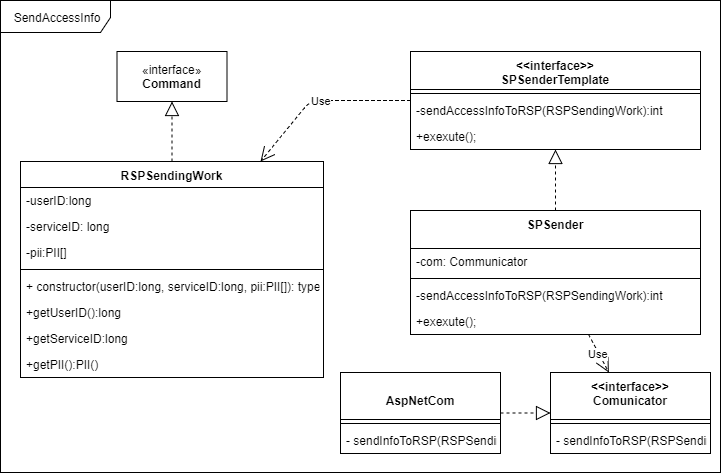
\includegraphics[width=0.9\columnwidth]{SendAccessInfo.png} 
    \caption{Rappresentazione UML di \emph{SendAccessInfo}}
    \label{fig:sendaccessinfo-uml-diag} 
\end{figure}

\begin{namespacedesc}
    \classdesc{RSPSenderTemplate}{questa interfaccia rappresenta il \emph{template} da seguire per eseguire il lavoro dell’esecutore. In altre parole rappresenta l’algoritmo da eseguire per espletare il lavoro di invio attributi al \emph{RSP}.}
    \classdesc{RSPSender}{questa classe implementa il \emph{template} da seguire per eseguire il lavoro dell’esecutore. In altre parole rappresenta l’algoritmo da eseguire per espletare il lavoro di invio attributi al \emph{RSP}.}
\end{namespacedesc}

\paragraph{CommonElement}
Questo componente contiene una serie di elementi usati da più esecutori, primi fra tutti gli oggetti \emph{Command}. Pertanto si è deciso di creare una libreria condivisa tra i vari esecutori.
Le classi più significative sono di seguito descritte.
 
\begin{namespacedesc}

    \classdesc{Command}{È una classe che rappresenta un generico evento nel contesto dell’architettura event driven. Questa interfaccia viene poi implementata da:
    \begin{itemize}
        \item \textbf{AccessRequest}: generato dallo starter e eseguito dal RetriveInfo, rappresenta il lavoro per gestire la richiesta di accesso;
        \item \textbf{PageResponce}: generato dal RetriveInfo in caso di errore o per mostrare il lettore QR, dal PiiDataHandler in caso di login o in caso di insuccesso della verifica. Rappresenta il lavoro di generazione e sottomissione delle pagine all’utente;
        \item \textbf{VerificationWork}: generato dallo Starter per verificare i dati forniti tramite il QR e quelli forniti da Monokee siano conformi e verificati; 
        \item \textbf{RSPSendingWork}: generato da PiiDataHandler in caso di verifica positiva. Rappresenta il lavoro di sottomissione dati in caso di verifica positiva.
    \end{itemize}
    }

    \classdesc{Hasher}{È un’interfaccia che ha il compito di eseguire l’hash di un dato. Rappresenta un’applicazione dello strategy pattern. }

    \classdesc{HasherImpl}{È una classe che implementa un’implementazione della classe Hasher. Esegue l’hash di un dato. Rappresenta con Hasher un’applicazione dello strategy pattern.}

\end{namespacedesc}


%**************************************************************
\subsection{Design Pattern utilizzati}
Al fine di garantire elevate doti di qualità e manutenibilità dell’architettura sono stati usati una serie di design pattern. Di seguito segue una breve descrizione di questi.


\paragraph{Command Pattern} permette di isolare la porzione di codice che effettua un'azione (eventualmente molto complessa) dal codice che ne richiede l'esecuzione; l'azione è incapsulata nell'oggetto Command. 
\paragraph{Remote Proxy} fornisce una rappresentazione locale di un oggetto remoto remote. 
\paragraph{Strategy Pattern} è un oggetto che permette di separare l’esecuzione di un metodo dalla classe che lo contiene. Usando un’interfaccia per astrarre il metodo è poi possibile crearne molteplici implementazioni. Questo è risultato molto utile nel contesto di un’applicazione multi piattaforma in cui alcune procedure andavano implementate in nativo. Oltre all’appena citato vantaggio questo ha reso possibile separare il metodo dall’implementazione. 
\paragraph{Dependency Injection} è un pattern che permette di delegare il controllo della creazione oggetti ad un oggetto esterno. Questo permette di semplificare la gestione delle dipendenze e nel contesto dello strategy pattern permette di inoculare l’implementazione corretta. 
\paragraph{Factory Method} è un pattern che permette di convogliare tutte le funzioni di creazione di vari elementi ad un oggetto unico. 

%**************************************************************
\section{Implementazione}

Le attività di implementazione e codifica sono state la parte di maggior impegno e sforzo dell'intero progetto. Hanno occupato in termini orari 120 ore, le quali rappresentano quasi il 40\% della durata del progetto. Esse hanno fatto emergere diversi errori di progettazione e di codifica, inoltre ci sono stati diverse ripensamenti da parte dell'azienda che hanno portato a riprogettare interi moduli. Nei paragrafi seguenti si cercherà di presentare le implementazioni più significative all'interno del progetto.

\subsection{Procedura di login}
L'applicativo mobile non prevedeva una gestione degli account propria, ma utilizzava gli account già presenti nel sistema Monokee. Questo ha necessitato quindi la codifica di un apposita procedura di login in modo di autenticare un utente in base ad una coppia di valori email e password. 

La suddetta procedura consiste principalmente in due chiamate HTTPS, la prima con lo scopo di ottenere l'id dell'utente tramite la mail fornita, la seconda allo scopo di verificare se la password sia conforne all'id ottenuto dalla prima chiamata. 

La prima fase era attuata da un metodo chiamato \textbf{Task<string> RetriveUserID(string usr)}. Questo metodo inviava tramite una POST il seguente json, con il quale forniva le informazioni necessarie ad ottenere l'id :

\begin{lstlisting}[caption={Json della prima request di login}]
    {
        email = "user@dominio.com",
        mobile = "false",
    }
\end{lstlisting}

La risposta doveva invece seguire il seguente schema:

\begin{lstlisting}[caption={Json risposta user\_id}]
    {
        success = "true",
        message = "ok",
        user_id = "df3c92kzz1",
    }
\end{lstlisting}

La risposta in alcuni casi poteva presentare altri campi dati, ma questi venivano ignorati dall'applicativo. Risposte che non presentavano le precedentemente citate tre informazione o che non riportavano i valori "true" ed "ok" rispettivamente su "success" e "message" causavano il lancio di un'eccezzione che faceva comparire un messaggio di fallimento a schermo.

Una volta ottenuto il valore "user\_id" si procedeva alla verifica della password col metodo
\textbf{getTokenID(string userId, string password)}.
Questo avveniva sempre tramite l'uso di una comunicazione POST. Nella request veniva mandato il seguente json:

\begin{lstlisting}[caption={Json richiesta token}]
    {
        user_id = "df3c92kzz1",
        password = "Passw0rd",
        mobile = "false",
        persistence = "false",
        cc_key = "key",
        salt = "salt",
        domain_id = "5b475bd150e783334b5bb861",
    }
\end{lstlisting}

Il campo "persistence" è utile alla gestione interna del dato e non rientra in nessun modo nel progetto.
I parametri "cc\_keys" e "salt" invece sono due valori tipici delle procedure di login. Questi servono a rendere più complessi gli attacchi a dizionario verso il sistema, infatti i due valori per essere generati richiedono un elevato onere computazionale sia in termini di spazio che di tempo, in quanto devono rispettare delle determinate condizioni. La codifica del codice per generare questi due valori ha richiesto innumerevoli sforzi e si è rivelata essere non banale.
L'applicativo Monokee ha la caratteristica di offrire ai propri utenti domini seperati, un tipico utilizzo di questi è per esempio il dominio aziendale e quello personale. Il "domain\_id" fornito da rappresenta il dominio personale. L'applicativo per ragioni di semplicità faceva l'accesso sempre allo stesso dominio. 

La risposta doveva seguire il seguente schema:
\begin{lstlisting}[caption={Json risposta token}]
    {
        success = "true",
        message = "ok",
        token = "qrdj99d7f9da0b2nf93Kd9LL"
    }
\end{lstlisting}

Il significato di "success" e "message" rimane analogo a quello precedentemente descritto, mentre il valore "token" rappresenta un codice da inserire nell'header sotto il nome di "Authorization" nelle successive chiamata in modo tale da essere risposto. Questo codice ha validità di 24 ore, al seguito delle quali scade ed è necessario rieffettuare la procedura di login. Risulta estremamente importante al momento del logout rimuovere dall'header il token, in quando una successiva operazione di login ne avrebbe aggiunto un altro causando un doppio token. Questo avrebbe fatto fallire le successive richiesta, seppur consentendo l'accesso.

Per ragioni progettuali interne a Monokee le chiamate se ricevute vengono sempre risposte con uno status code 200, a prescindere del fatto che queste siano accettate o rifiutate. Per questa ragione al fine di sostituire i vari codici di errore vengono usati i campi "success" e "message". 

La codifica di questa procedura non ha presentato particolari difficolta se non quella della generazione del cc\_key e del salt. 

\subsection{Uso del database SQLite}

Nel contesto dell'applicazione mobile per effettuare la persistenza dei dati si è deciso di utilizzare una base di dati relazionale. La scelta è ricaduta su SQLite. Si è deciso di operare con questa base di dati utilizzando il design pattern \emph{data access object} e apposite libreria di sistema che lo implementavano, questa pratica si è rivelata essere molto pratica ed efficace ai fini del progetto. Ovviamente risulta limitata comparata rispetto all'uso del codice \emph{sql}, ma le necessità applicative non richiedevano simili finezze.

A titolo di esempio si discute ora della memorizzazione di un PII.

\begin{lstlisting}[caption={codice creazione DAO}]
    public DBDao()
    {
        database = DependencyService
            .Get<ILocalDataProvider>()
            .GetConnection();
        database.CreateTable<PIIModel>();
        database.CreateTable<UserModel>();
    }
\end{lstlisting}

Il codice appena presentato rappresenta la creazione dell'oggetto che fornisce l'accesso alla base di dati, come si può notare il corpo del costrutture crea una connessione tramite l'uso di \emph{DependencyService}, successivamente crea le tabelle. Ovviamente in caso le tabelle siano già presenti, le istruzioni non alterano la base di dati. 

A differenza di quanto uno si potrebbe aspettare, la funzione \emph{CreateTable} non richiede informazione sui tipi di dato e/o sulle colonne da creare. Queste informazione vengono dedotte dal tipo che gli viene fornito, il quale andrà a rappresentare il modello di una tupla della tabella.

Si propone adesso il codice di \emph{PIIModel}:
\begin{lstlisting}[caption={codice PIIModel}]
    [Table("PIIModel")]
    public class PIIModel
    {
 
        [PrimaryKey, AutoIncrement]
        public int Id;
        
        [Indexed(Name = "nameId", Order = 1, Unique = true)]
        public string UserID;

        [Indexed(Name = "nameId", Order = 2, Unique = true)]
        public string Name;
        [NotNull]

        //continua ...
\end{lstlisting}

I campi dati pubblici vengono considerati come i valori delle colonne, mentre altre informazioni necessarie vengono fornite tra parentesi quadre. Queste sono per esempio le chiavi, i valori non nulli, i vincoli di integrità, il nome della tabella etc...

Sequendo questa tecnica la gestione del database risulta particolarmente semplice. Vengono ora riportati degli esempi di codice per l'inserimento e la rimozione di una PII dalla base di dati:

\begin{lstlisting}[caption={codice aggiunta e rimozione PIIModel}]
public int AddPII(PIIModel pii)
    {
        lock (collisionLock)
        {
            if (pii.Id != 0)
            {
                database.Update(pii);
                return pii.Id;
            }
            else return database.Insert(pii);      
        }
    }

public int DeletePII(int piiID)
{
    lock(collisionLock)
    {
        return database.Delete<PIIModel>(piiID);
    }
}
\end{lstlisting}

Ovviamente query più complicate risultano non essere possibile tramite funzioni di libreria, per queste particolari occassioni si è dovuto utilizzare del codice sql.

\begin{lstlisting}[caption={Esempio di query sql}]
public List<PIIModel> GetPIIs(string name, string user\_id)
    {
        lock (collisionLock)
        {
            return (from i in database.Table<PIIModel>()
                    where (i.Name == name && i.UserID==user\_id)
                    select i).ToList();
        }
    }
\end{lstlisting}

L'uso di queste tecniche e dei modelli ha permesso di limitare al massimo l'utilizzo di codice sql, inoltre ha permesso una più facile gestione del dato in quanto la risposta ad una query veniva già presentata in forma di oggetto.

\subsection{Implementazione del databinding}
L'applicaione mobile richiedeva la creazione di molteplici schermate che dovevano sempre rimanenere aggiornare rispetto ad un particolare oggetto e viceversa. Questo risultava particolarmente importante in quanto era fondamentale che l’interfaccia fosse ben separata dalla logica di business, affinché una modifica nella logica o nel modello di dominio non si rifletta sull’interfaccia. 

A questi scopi \emph{Xamarin} offre la cosidetta tecnica del databinding tra intefaccia e oggetto. Ora si ripropone l'oggetto PIIModel, questa volta però non omettendo il codice necessario per il databinding.

\begin{lstlisting}[caption={esempio di oggetto in databinding}]
[Table("PIIModel")]
public class PIIModel : INotifyPropertyChanged
{
    private int piiID;
    [PrimaryKey, AutoIncrement]
    public int Id
    {
        get { return piiID; }
        set {
            piiID = value;
            OnPropertyChanged(nameof(Id));
        }
    }

    \\altro codice ommesso ...

    private void OnPropertyChanged(string propertyName)
    {
            PropertyChanged?.Invoke(this,
            new PropertyChangedEventArgs(propertyName));
    }
}
\end{lstlisting}

Come si può notare per poter effettuare il databinding è necessario che la classe PIIModel implementi l’interfaccia INotifyPropertyChanged, che definisce l’evento PropertyChanged di tipo PropertyChangedEventHandler. Questo evento prende un’istanza della classe PropertyChangedEventArgs che definisce la proprietà PropertyName di tipo string, attraverso la quale è possibile sapere quale proprietà nell'oggetto PIIModel è cambiata (permettendo all’evento di accedere a quella proprietà).

Attraverso la proprietà pubblica Id, offriamo la possibilità lato codice di ottenere le informazioni sul valore corrente attraverso il get, e di impostare un nuovo valore per tale proprietà attraverso il set ogni qualvolta il valore assunto dalla variabile name differisce da quella corrente. Proprio in quest’ultima porzione viene richiamato il metodo OnPropertyChanged, che prenderà in ingresso il nome della proprietà che deve essere aggiornata innescando il meccanismo sopra descritto. 

Per effettuare l'effettiva collegamento basta inserire nel codice che gestische la schermata la seguente istruzione:
\begin{lstlisting}[caption={codice di connessione}]
    BindingContext = PIIModel;
\end{lstlisting}

Questo renderà possibile nel codice grafico (XAML) di poter utilizzare i valori dell'oggetto. Di seguito viene mostrato un esempio:

\begin{lstlisting}[caption={esempio di vista che usa il databinding}]
<?xml version="1.0" encoding="utf-8" ?>
<ContentPage xmlns="http://xamarin.com/schemas/2014/forms"
             xmlns:x="http://schemas.microsoft.com/winfx/2009/xaml"
             x:Class="IdentityWallet.PIIVisualizerPage"
             Title="{Binding Name}">
    <ContentPage.Content>
        <ScrollView>
            <StackLayout VerticalOptions="StartAndExpand" Padding="20">
                <Label Text="Id"/>
                <Label x:Name="piiID" Text="{Binding Id}"/>
            
                <Label Text="Name" />
                <Entry x:Name="piiName" Text="{Binding Name}"/>
            
                <- altro codice ->
            </StackLayout>
        </ScrollView>
    </ContentPage.Content>
</ContentPage>
\end{lstlisting}

\subsection{Instaurazione della rete di messaggi}
Il modulo SP è composto da diversi componenti, i quali sono residenti in programmi differenti e seperati fra loro. L'unico modo di comunicazione che utilizzano è un \gls{messagebrokerg}\glsfirstoccur di nome \emph{RabbitMQ}. Questo deve essere eseguito su un server e verrà utilizzato dai vari componenti tramite il suo \emph{uri}.
L'applicativo richiede che nel server sia installato \emph{Erlang}. Una volta averlo installato si può procedere all'installazione di \emph{RabbitMQ} seguendo la guida presente al seguente url \url{https://www.rabbitmq.com/download.html}. Per eseguire correttamente le funzionalità del modulo SP è inoltre necessario creare una rete col nome di "test"; per fare questo è necessario abilitare l'interfaccia di configurazione di \emph{RabbitMQ} seguendo la seguente guida \url{https://www.rabbitmq.com/management.html}.
Una volta abilitata l'interfaccia questa sarà disponibile al seguente indirizzo \url{http://localhost:15672/#/connections}. La pagina che si presenterà avrà una scheda chiamata "network" dalla quale sarà possibile aggiungere la rete di nome "test".
Fatto questa la configurazione di \emph{RabbitMQ} è terminata; ora basta avviare il broker tramite terminale usando il comando \emph{rabbitmq-server start}.


\subsection{Gestione delle code e dei messaggi}
Come già discusso il modulo SP ha un'architettura del tipo \emph{even driven}. L'applicazione di tale libreria ha necessitato dell'uso di una libreria per la gestione e l'invio dei vari messaggi.

Il modulo SP è diviso in molteplici esecutori ognuno del quale presente del codice per la gestione dei messaggi equivalente, a titolo di esempio si procede ad esporre l'esecutore \emph{ITFVerifier}.

All'avvio l'esecutore ha il compito di creare un oggetto in grado di individuare la rete che gestisce i messaggi (questa era disponibile all'uri definito in \emph{GeneralSetting.RabbitMQHost}) e quindi effettuare il collegamento ad essa tramite la sottomissione di una coppia username, password.
Successivamente era necessario definire cosa doveva essere fatto dei messaggi in arrivo e sopratutto quale tipo di messaggi dovessero essere ascoltati. La parte finale del codice propostro mostra le instruzione necessarie a fare quanto appena detto. Tramite \emph{ReceiveEndpoint} viene stabilito il nome della coda dove verranno inseriti i messaggi catturati e il comportamento da intraprendere per ognuno di questi messaggi. Come comportarsi viene definito tramite una arrow function che instanzia un \emph{Consumer} con un tipo da noi definito (\emph{VerificationWorkConsumer}). I messaggi da inserire nella code di ricezione non vengono decisi in base ad un'indicazione del mandante, ma tramite il tipo dell'oggetto che implementa \emph{VerificationWorkConsumer}.
L'ultimi riga ha lo scopo di eseguire il lavoro in modalità asincrona.
\begin{lstlisting}[caption={creazione di un collegamento a \emph{RabbitMQ}}]
    _busControl = Bus.Factory.CreateUsingRabbitMq(x =>
        {
            IRabbitMqHost host = x.Host(new Uri(GeneralSetting.RabbitMQHost), h =>
            {
                h.Username("guest");
                h.Password("guest");
            });
            
            x.ReceiveEndpoint(host, "VerQueue",
                e => { e.Consumer<VerificationWorkConsumer>(); });
            
        });

        TaskUtil.Await(() => _busControl.StartAsync());
\end{lstlisting}

Adesso risulta utile analizzare il codice del \emph{Consumer}. Come si può notare la classe implementa \emph{IVerificationWork}, pertando nella coda che porta il nome di "VerQueue" verranno inseriti solo i messaggi che hanno come tipo \emph{IVerificationWork}.
Unico metodo implementabile è \emph{Consume} il quale rappresenta il codice da effettuare.

\begin{lstlisting}[caption={esempio di \emph{Consumer}}]
public class VerificationWorkConsumer : IConsumer<IVerificationWork>
{
    public async Task Consume(ConsumeContext<IVerificationWork> context)
    {
            //operazioni da effettuare

    }
}
\end{lstlisting}

Andiamo ora a vedere come si invia un messaggio un \emph{VerificationWork}:
\begin{lstlisting}[caption={codice invio di un messaggio}]
    public async Task SendToVerificationAsync(IVerificationWork verWork)
    {
        await _busControl.Publish(verWork);
    }
\end{lstlisting}

Come potete vedere questo avviene tramite la funzione \emph{Publish} dell'oggetto \emph{\_busControl}.

\subsection{Interazioni con la \emph{blockchain}}

Sia l'applicativo mobile IW, che l'applicativo server SP hanno previsto l'uso della stessa libreria \emph{Nethereum} al fine di effettuare le necessarie chiamate alla \emph{blockchain Ethereum}.
Questa libreria implementa il protocollo Ethereum\footcite{site:ethereum-yellow-paper} in ambiente \emph{.NET}.

Il protocollo discerne tra due tipi di chiamate, quelle in \textbf{sola lettura} e quella \textbf{in scrittura}; le prime sono identificate dai modificatori \emph{pure} o \emph{view}.

Le chiamate in sola lettura sono immediate e non richiedono l'esecuzione di una transazione, per queste ragioni hanno prestazione paragonabile a quelle di un linguaggio tradizionale e non richiedono le venga fornito dell'\gls{etherg}.

Le seconde invece, dovendo modificare la blockchain, hanno bisogno di effettuare una transazione con la conseguente esecuzione dell'algoritmo di consenso descritto nel capitolo \ref{cap:alg-cons}. Questo porta ai problemi di prestazioni e costo descritti in \ref{cap:prestazioni}

Prima di poter procedere a qualsiasi operazione era necessario creare un collegamente alla rete \emph{Ethereum} usata (nel nostro caso una rete locale all'azienda). Il sequente codice mostra le istruzioni necessarie.

\begin{lstlisting}[caption={Connessione alla rete di test},label={lst:connessione},language={C}]
account = new Account(GeneralSetting.accountPrivKey);
web3 = new Web3(account, blockchain_address);
\end{lstlisting}

La variabile \emph{web3} è l'oggetto che rappresenta la connessione. Il primo parametro del costruttore non è strettamente necessario, ma stabilisce un account di default con il quale verranno pagate le transazioni. Si è deciso in fase di codifica di non minare direttamente le aggiunte di blocchi, ma di pagare la transazione. Per essere riconosciuti dalla rete è sufficiente fornire la chiave privata. 
\medskip

Ora è necessario richiamare un contratto presente nella rete. Per fare questo necessitiamo di due informazione: l'\textbf{indirizzo} e l'\gls{abig}\glsfirstoccur. L'\emph{ABI} di un contratto consiste in un json contenente la definizione di tutti i metodi presenti nel contratto. Nel frammento ~\ref{lst:abi_ex} si mostra l'\emph{ABI} della chiamata che andremo ad effettuare, invece nel frammento ~\ref{lst:creazioneContr} si mostra la creazione dell'oggetto contratto. Dal contratto poi si ottiene la funzione.

\begin{lstlisting}[caption={Esempio di ABI},label={lst:abi_ex},language={C}]
[
    {
        "anonymous": false,
        "inputs": [
            {
                "indexed": true,
                "name": "_PII_ID",
                "type": "string"
            },
            {
                "indexed": false,
                "name": "result",
                "type": "bool"
            }
        ],
        "name": "eventResponse",
        "type": "event"
    },
    {
        "constant": false,
        "inputs": [
            {
                "name": "_publicKey",
                "type": "string"
            },
            {
                "name": "_PII_ID",
                "type": "string"
            },
            {
                "name": "_name",
                "type": "string"
            },
            {
                "name": "_description",
                "type": "string"
            }
        ],
        "name": "verify",
        "outputs": [
            {
                "name": "",
                "type": "bool"
            }
        ],
        "payable": false,
        "stateMutability": "nonpayable",
        "type": "function"
    }
]  
\end{lstlisting}

\begin{lstlisting}[caption={Creazione del contratto},label={lst:creazioneContr},language={[Sharp]C}]
    SPFContract = web3.Eth.GetContract(abi,
                "contract_address");
    var verifyFunction = SPFContract.GetFunction("verify");
\end{lstlisting}

Una volta ottenuto l'oggetto \emph{verifyFunction} non ci resta che effettuare la chiamata. Il metodo \emph{verify} effettua modifiche, quindi è necessario effettuare una transazione. La funzione \emph{SendTransactionAndWaitForReceiptAsync} effettua la chiamata del metodo solidity \emph{verify} e aspetta che questa fallisca o abbia successo. Una transazione non restituisce mai il risultato della chiamata, ma una ricevuta che ne attesta la riuscita o il fallimento. Per ottenere il risultato bisogna usare i cosidetti \emph{eventi} che vanno lanciati dal codice solidity con il contenuto del valore di ritorno. Gli eventi sono comunicati in \emph{broadcast} a tutti gli utenti connessi alla rete, di conseguenza ottenere il risultato richiede una serie di procedure particolari. La seconda parte del codice nel frammento  \ref{lst:transax} mostra il codice necessario per filtrare gli eventi in base alla ricevuta e quindi ottenere il valore. 


\begin{lstlisting}[caption={Creazione del contratto},label={lst:transax},language={[Sharp]C}]
receipt = await verifyFunction.SendTransactionAndWaitForReceiptAsync(
    "account_address,
    null, 
    ITFID,
    description, 
    publicKeyBytes)
    .ConfigureAwait(false);          

    //CODICE PER GESTIRE L'EVENTO DI RISPOSTA
    var verifyEvent = SPFContract.GetEvent("eventResponse");
    var filterOnITFID = verifyEvent.CreateFilterInput(
        new BlockParameter(receipt.BlockNumber),
            BlockParameter.CreateLatest());
    var log = await verifyEvent.GetAllChanges<VerificationEvent>(filterOnITFID);
    result = log[0].Event.Result;
\end{lstlisting}


Le chiamate a metodi solidity detti \emph{puri}, invece, sono più semplici e restituiscono direttamente il risultato.
Di seguito un esempio di una chiamata di questo tipo.

\begin{lstlisting}[caption={Esempio di chiamata a metodo puro},label={lst:call_ex},language={[Sharp]C}]

getFunction = SPFContract.GetFunction("getFromID");
string result = await getFunction.CallAsync(par1, par2);
    
\end{lstlisting}


\subsection{Procedura di accesso a servizio}
Di seguito viene esposte le varie azione che vengono scatenate durante una tipica operazione di accesso ad un servizio. Il progetto è compatibile con tutti i servizi compatibili con lo standard \gls{samlg}.

\noindent Si propone come esempio l'applicativo \emph{Salesforce}.

Tramite l'interfaccia di \emph{Salesforce} abbiamo creato un apposito dominio di accesso. In questo modo l'utente potrà in fase di login specificare il dominio con il quale effettuare l'accesso.
Le immagini \ref{fig:salesforce-login} e \ref{fig:salesforce-dom} mostrano come indicare il dominio.

\begin{figure}[!h]
    
    \centering
    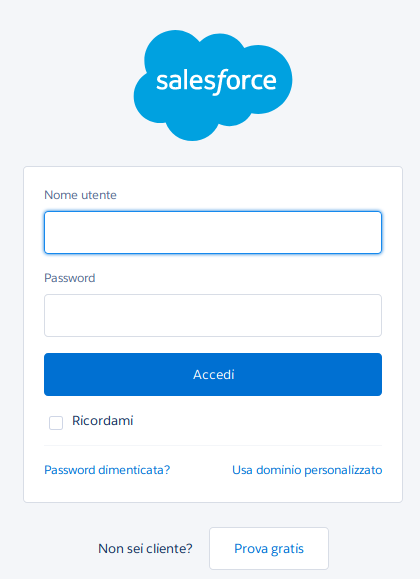
\includegraphics[width=0.4\columnwidth]{login.png} 
    \caption{Schermata di login di Salesforce}
    \label{fig:salesforce-login} 
\end{figure}

\begin{figure}[!h]
    
    \centering
    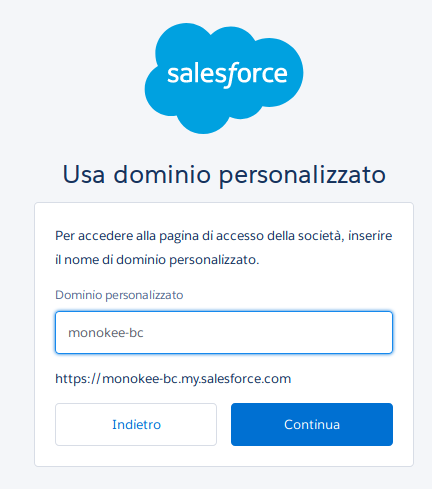
\includegraphics[width=0.4\columnwidth]{dominioLogin.png} 
    \caption{Schermata di scelta dominio}
    \label{fig:salesforce-dom} 
\end{figure}

Indicando il dominio corretto il browser procederà a reindirizzare l'utento presso un apposito sito interno al \emph{back-end} di Monokee.

L'inoltro verso il sito scatenerà le seguenti operazioni:
\begin{enumerate}
    \item collegamento verso un canale \gls{websocketg} gestito dal componente \emph{ResultSender} del modulo SP;
    \item attivazione della web-cam del computer e cattura di immagini fino all'individuazione di un codice QR compatile con quello generato dall'applicativo mobile IW;
    \item invio tramite comunicazione POST del contenuto del codice QR al modulo SP, la risposta alla POST conterrà un \gls{nonceg} da usare in seguito;
    \item verifica da parte del componente SP delle informazioni di accesso fornite tramite la POST e quindi invio del risultato e del \emph{nonce} tramite il canale \emph{WebSocket}. Il componente SP si occuperà inoltre di comunicare l'esito anche al \emph{back-end} di Monokee, il quale si occuperà della generazione della \emph{SAMLResponse}\footnote{La SAMLResponse consiste in \emph{XML} contenente tutte le informazioni necessarie a Salesforce per permettere l'accesso. Volendo fare un esempio nel caso di un servizio che richieda username e password, l'\emph{XML} conterrà questi due dati con l'aggiunta di una serie di firme e informazione utili a garantire la sicurezza del protocolo. Per maggiori dettagli consultare \url{https://www.samltool.com/generic_sso_res.php}.} corrispondente;
    \item inserimento della \emph{SAMLResponse} da parte del \emph{back-end} di Monokee all'interno di una form presente nel sito;
    \item ricezione da parte del sito dell'esito della verifica tramite il canale \gls{websocketg};
    \item verifica dell'uguaglianza del \emph{nonce} ricevuto dalla POST con quello ricevuto dall'esito della verifica e verifica della positività dell'esito ;
    \item in caso entrambe le verifiche abbiamo riscontro positivo invio tramite POST della \emph{SAMLResponse} al \emph{back-end} di Salesforce;
    \item reindirizzamento verso l'applicativo Salesforce. Ora si è riconosciuti come utenti.
\end{enumerate}

\noindent Qualora una qualsiasi delle precedenti operazioni fallisse o desse esito negativo il sito mostrerà un messaggio di errore a schermo e richiederà la risottimissione del codice QR.
